\documentclass{article}

\usepackage{microtype}
\usepackage{graphicx}
\usepackage{subcaption}
\usepackage{booktabs}
\usepackage{array}
\usepackage{multirow}
\usepackage{xcolor}
\usepackage{amsmath}
\usepackage{amssymb}
\usepackage{mathtools}
\usepackage{natbib}
\usepackage{hyperref}
\newcommand{\theHalgorithm}{\arabic{algorithm}}
\usepackage[accepted]{icml2026}

\icmltitlerunning{Token-Level Verification under Controlled Evaluation}

\begin{document}

\twocolumn[
\icmltitle{Token-Level Verification under Controlled Evaluation:\\ Protocol Sensitivity Shapes Apparent Performance}

\begin{icmlauthorlist}
  \icmlauthor{Yuhan Chi}{fudan}
\end{icmlauthorlist}

\icmlaffiliation{fudan}{School of Mathematical Sciences, Fudan University, Shanghai, China}
\icmlcorrespondingauthor{Yuhan Chi}{yhchi25@m.fudan.edu.cn}
\icmlkeywords{AI for Math, Verification, Uncertainty, Evaluation Protocols, Large Language Models}

\vskip 0.3in
]

\printAffiliationsAndNotice{Code: \url{https://github.com/Chi-Shan0707/token-verification-mirage}. }

\begin{abstract}
Token-level uncertainty signals such as entropy, log-probabilities, and confidence scores are increasingly explored as lightweight aids for verifying LLM reasoning without additional model calls. Yet reported AUROC varies from near-chance (0.55) to high values (0.80+), with no consensus on what drives this variance. Prior work has not systematically isolated, within this math-verification setting, how much of this variation stems from evaluation protocol artifacts rather than genuine signal differences.

We conduct a controlled study across two benchmarks (MATH, BigMath), two model families (Qwen, Llama; three instances), and twelve analytical methods under within-problem leave-one-out (LOO) evaluation, GroupKFold cross-problem splits, and permutation-null calibration.

We find that evaluation protocol choices can shift AUROC more than the observed differences among several methods in our setting; switching from pooled to within-problem LOO evaluation shifts AUROC by 0.04--0.18. Under controlled evaluation, all twelve analyzed methods converge to an overlapping AUROC range of roughly 0.60--0.75 on hard math problems, with genuine excess above the permutation null ($\approx$0.58--0.60) of only $\approx$0.05--0.15. Direction-agnostic (DA) scoring---selecting the better scoring direction per problem---yields this range, but a fixed-direction baseline (learning one global direction) reveals that final-token entropy collapses from 0.72--0.75 to 0.47--0.48 (below chance), indicating its apparent strength reflects per-problem direction selection rather than stable generalization. Two adapted prior token-level uncertainty baselines~\cite{wang2025eat,malinin2021uncertainty} fall within the same range; a Kadavath-style P(True) self-evaluation baseline~\cite{kadavath2022language} achieves higher AUROC than these shallow statistics under the same direction-agnostic evaluation. The accompanying repository provides the evaluation scripts and paper artifacts.
\end{abstract}
\section{Introduction}
\label{sec:intro}

In math-reasoning systems, \textit{verification} asks whether sampled solutions can be ranked by correctness without additional expensive evaluation~\cite{hendrycks2021measuring,cobbe2021gsm8k}. In full AI-for-math systems, this role is often served by stronger mechanisms such as symbolic checking, code or tool execution, learned verifiers, reward models, process supervision, or self-consistency. These approaches can be effective but may require additional model calls, labeled data, external tools, or fine-tuning. Lightweight alternatives extract verification signals directly from the token-level statistics already produced during generation---entropy, log-probabilities, and confidence trajectories---without any additional model calls~\cite{wang2025eat,malinin2021uncertainty}. A related but richer family of approaches prompts the model to evaluate its own answer, e.g. P(True) self-evaluation~\cite{kadavath2022language}.

This premise has motivated a growing line of work. Wang et al.~\cite{wang2025eat} use entropy-after-thinking signals for reasoning-model early exit; we adapt this entropy-trajectory idea as one lightweight uncertainty baseline. Malinin \& Gales~\cite{malinin2021uncertainty} derive token-level uncertainty decompositions from ensemble distributions. Kadavath et al.~\cite{kadavath2022language} show that models can self-assess answer correctness via P(True) prompts. Self-consistency reranking~\cite{wang2023selfconsistency} uses answer agreement across samples. Process reward models~\cite{lightman2023let,uesato2022solving} and neuron-agreement analyses~\cite{chen2025nad} access richer supervision or internal signals. These methods span a wide design space; our controlled study focuses on the shallow external token-statistic end of that space.

Reported results, however, are inconsistent. AUROC values for token-level verifiers span 0.55--0.80+ across studies, with no consensus on whether this variation reflects genuine methodological advances or evaluation artifacts. This makes it difficult to assess whether additional verification features improve over simple baselines.

Our experiments indicate that evaluation design is a major contributor to the observed variation. Global pooled evaluation---pooling predictions across problems---conflates problem-level difficulty with solution-level correctness, allowing a verifier to exploit problem-level difficulty signals rather than genuine per-solution discrimination, shifting AUROC by 0.04--0.18 relative to within-problem evaluation. In-sample evaluation of within-problem methods introduces subtle leakage: using a held-out trace's neighbors to construct scoring centroids biases AUROC estimates. These two protocol artifacts, taken together, can shift measured AUROC by 0.04--0.18 (Table~\ref{tab:protocol}), an effect that exceeds the entire range of genuine method-driven variation under controlled evaluation.

Instead of proposing a new verification method, we audit what shallow external token statistics can extract under controlled evaluation. This diagnostic focus is deliberate: before token-level signals are used as low-cost filters, auxiliary rerankers, or baselines for stronger verifiers, their evaluation protocol must not overstate their standalone discriminative power. We enforce three methodological controls: (i) within-problem LOO evaluation that eliminates problem-identity leakage; (ii) GroupKFold by problem for cross-problem analyses; and (iii) permutation-null calibration that accounts for direction-agnostic scoring inflation. Under this protocol, we benchmark twelve analytical methods across two model families and two benchmarks, and implement three prior-inspired baselines to check whether related uncertainty and self-evaluation signals fall in the same range.

In our experiments, protocol choice has a larger effect than feature design on reported performance. Under controlled evaluation, the analyzed methods occupy a narrow DA AUROC range of 0.60--0.75 on hard problems, with bootstrap CIs that substantially overlap. A key practical distinction emerges between oracle and fixed-direction evaluation: final-token entropy achieves the highest DA AUROC but collapses to chance (0.47--0.48) under fixed-direction AUROC, because the entropy-correctness direction varies idiosyncratically across problems. The prior-inspired baselines fall within or above the same range, with the Kadavath-style semantic self-evaluation baseline achieving higher AUROC than shallow token statistics under direction-agnostic scoring.

Our primary contribution is an empirical evaluation framework that makes protocol-induced inflation explicit and reproducible. Our practical contribution is a set of protocol recommendations and analysis code for future work, especially for studies that report lightweight token-level signals as baselines or as components of larger verification pipelines. Figure~\ref{fig:overview} summarizes the core findings.

\begin{figure*}[t]
\centering
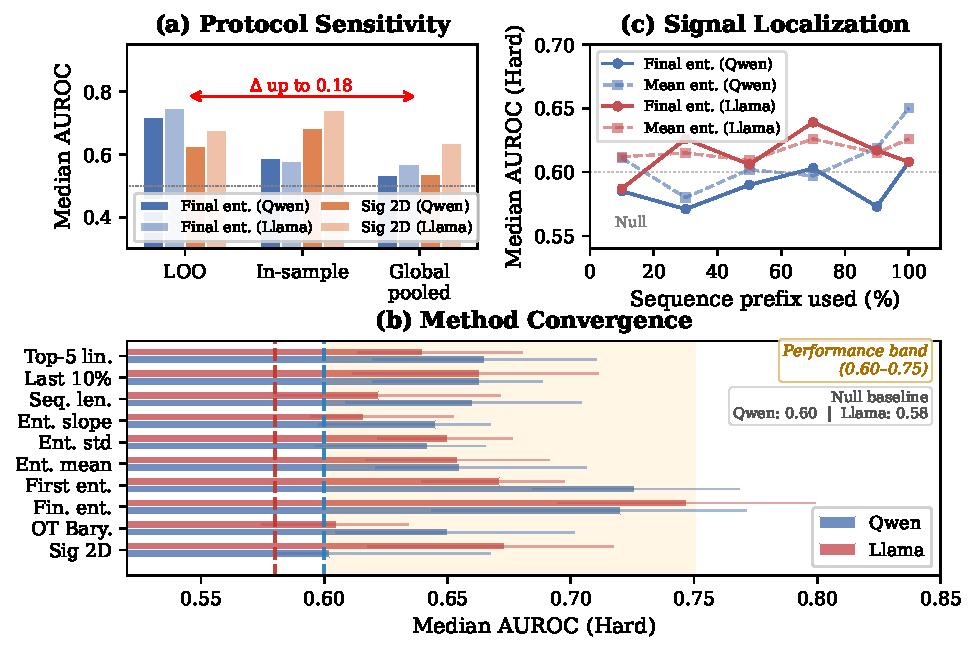
\includegraphics[width=0.98\textwidth]{fig_overview_icml.pdf}
\caption{Overview of core findings. \textbf{(a)} Median AUROC under three evaluation protocols. \textbf{(b)} Hard-problem AUROC of all methods under LOO, with permutation-null baselines. \textbf{(c)} Prefix-based ablation showing how performance changes with sequence coverage.}
\label{fig:overview}
\end{figure*}

\section{Related Work}
\label{sec:related}

\textbf{Outcome and process reward models.} Outcome reward models (ORMs) train binary classifiers on complete solution traces~\cite{cobbe2021gsm8k}. Process reward models (PRMs) extend this to step-level verification~\cite{lightman2023let,uesato2022solving}, showing that fine-grained supervision improves verification accuracy. Both require substantial labeled data and model fine-tuning. Our work focuses on the complementary question: what can token-level statistics available from generation metadata---already available from generation---provide without any training?

\textbf{Token-level uncertainty methods.} Several lines of work extract uncertainty or verification-related signals from generation metadata. Wang et al.~\cite{wang2025eat} study entropy-after-thinking signals for reasoning-model early exit; in our experiments we adapt the resulting entropy-trajectory intuition to within-problem correctness ranking. Malinin \& Gales~\cite{malinin2021uncertainty} decompose token-level uncertainty into total, data, and knowledge uncertainty (mutual information) using ensemble disagreement. Self-consistency reranking~\cite{wang2023selfconsistency} uses answer agreement as a proxy for correctness. A different approach is taken by Kadavath et al.~\cite{kadavath2022language}, who demonstrate that models can self-assess via P(True) prompts with few-shot examples. These methods are evaluated under heterogeneous protocols---including global pooling and in-sample evaluation---and generally do not report the combination of within-problem LOO, fixed-direction AUROC, and permutation-null calibration used here, making cross-study comparison unreliable.

\textbf{Internal vs.\ external signals.} Chen et al.~\cite{chen2025nad} study neuron-agreement signals as internal evidence of whether LLM answers are correct. This line of work raises a complementary question: what do external token statistics retain when internal activations are unavailable? We quantify this narrower external-signal setting under controlled evaluation.

\textbf{Evaluation methodology.} Our contribution is to quantify these evaluation-protocol choices for shallow token-level math-reasoning verification. We use path signatures~\cite{lyons1998differential,chen1958integration,kidger2019deep,chevyrev2016primer} and optimal transport~\cite{peyre2019computational} as diagnostic probes to map the performance envelope.

\section{A Motivating Example}
\label{sec:motivation}

\begin{figure}[t]
\centering
\fbox{\parbox{0.92\columnwidth}{\small\textbf{Problem:} A fair six-sided die is rolled 720 times. What is the expected number of times that a prime number appears?

\textbf{Solution A} (correct, entropy 0.012): ``The prime numbers on a six-sided die are 2, 3, and 5, so $p = 3/6 = 1/2$. Expected count: $720 \times 1/2 = \boxed{360}$.''

\textbf{Solution B} (incorrect, entropy 0.008): ``Primes: 2, 3, 5. $E[X] = np = 720 \times 3/6 = \boxed{1080}$.''

\textbf{Solution C} (incorrect, entropy 0.341): ``The probability of getting a prime is $3/6 = 1/2$. We need to count the primes in 720 rolls... The answer is $\boxed{480}$.''}}
\caption{Motivating example. Solutions A (correct) and B (incorrect) both produce very low entropy, while C (incorrect) produces high entropy. The key point is that low entropy can accompany confident errors (B), so a single global direction for entropy-based verification is unreliable.}
\label{fig:motivation}
\end{figure}

Figure~\ref{fig:motivation} illustrates the fundamental challenge. On the same math problem, a correct solution and an incorrect solution can both produce very low final-token entropy when the model is confident in its (possibly wrong) answer. Conversely, an incorrect solution can produce high entropy when the model is genuinely confused. A token-level verifier faces an inherently noisy signal: the entropy-correctness relationship varies across problems, and no single global direction (``higher entropy = more likely wrong'') holds universally.

We therefore evaluate the discriminative capacity of shallow token statistics after removing these artifacts. This requires an evaluation protocol that does not itself inflate or distort the observed signal.

\section{Standard Evaluation Protocol}
\label{sec:sep}

For clarity and reproducibility, we use the following six evaluation controls:

\textbf{Step 1: Data Collection \& WP-Eligibility Filter.} For each problem, collect $N$ independent generations (we use $N{=}64$, nucleus sampling $p{=}0.95$, temperature 0.6). Filter to within-problem eligible (WP-eligible) problems: those with $\geq 2$ correct and $\geq 2$ incorrect runs. This filtering is necessary for LOO evaluation and introduces a conditional subset bias.

\textbf{Step 2: Within-Problem Leave-One-Out (LOO).} For each problem, hold out one run as test; construct scoring centroids from the remaining correct and incorrect runs. This eliminates problem-identity leakage.

\textbf{Step 3: GroupKFold by Problem.} For cross-problem analyses, split by problem ID (not runs) using GroupKFold ($K{=}5$), preventing the model from learning problem-specific difficulty.

\textbf{Step 4: Direction-Agnostic Scoring with Permutation-Null Calibration.} Report per-problem $\max(\text{AUROC}, 1{-}\text{AUROC})$, which is an \textit{oracle upper bound} on separability. Compute permutation null via 1000 label permutations per problem; the null is $\approx$0.58--0.60 (not 0.5). Report both DA and fixed-direction results (Step 6).

\textbf{Step 5: Per-Difficulty Stratification with Bootstrap CI.} Report results stratified by difficulty tier. Compute median and 95\% CI via 10,000 problem-level bootstrap resamples.

\textbf{Step 6: Fixed-Direction Baseline.} Learn a global scoring direction from GroupKFold training folds; evaluate on held-out problems. This provides a non-oracle estimate of practical verifier performance. Report alongside DA results.

\section{Experimental Setup}
\label{sec:setup}

\subsection{Datasets and Models}

\begin{table}[t]
\centering
\caption{Datasets and models. WP-elig.\ = within-problem eligible ($\geq 2$ correct, $\geq 2$ wrong).}
\label{tab:datasets}
\resizebox{\columnwidth}{!}{%
\begin{tabular}{lccccc}
\toprule
Dataset & Model & Arch. & Traces & Accuracy & WP-elig. (H/M/E) \\
\midrule
MATH & Qwen3-32B & Qwen & $\sim$11.7K & 7--98\% & 365 total \\
BigMath & Qwen2.5-Coder-7B & Qwen & 25,600 & 55.3\% & 62/70/47 \\
BigMath & Llama-3.1-8B & Llama & 25,600 & 39.3\% & 64/101/83 \\
\bottomrule
\end{tabular}%
}
\end{table}

Three model instances across two architecture families (Table~\ref{tab:datasets}). BigMath is our curated subset of 400 problems from the Open-R1 dataset~\cite{openr1bigmath}, including MATH~\cite{hendrycks2021measuring}, Orca Math~\cite{mukherjee2023orca}, and GSM8K~\cite{cobbe2021gsm8k}. Difficulty tiers are stratified by Llama-8B solve rate. We collect 64 independent generations per problem; correctness is determined by exact match of the extracted final answer.

\subsection{Methods}

\textbf{Scalar baselines}: entropy mean, std, final-token entropy, first-token entropy, slope, sequence length, last-10\%-mean.

\textbf{Temporal methods}: Path signatures (depth-3, 2D $[t, \text{entropy}]$, 15 dimensions, LOO centroid-distance scoring).

\textbf{Distributional methods}: OT Barycenter (1D Wasserstein, quantile space, LOO scoring).

\textbf{Spectral/transition methods}: Fourier spectral (4D) and Markov 4-state transition matrix (16D), described and evaluated in Appendix~\ref{app:spectral}.

\textbf{Cross-problem learned verifier}: 3-layer MLP (6 features $\to$ 64 $\to$ 32 $\to$ 1), GroupKFold 5-fold.

\section{Results}
\label{sec:results}

\subsection{Evaluation Protocol Artifacts Account for the Largest Share of Reported Variation}
\label{sec:protocol}

\begin{table}[t]
\centering
\caption{Effect of evaluation protocol on hard-problem AUROC. Negative $\Delta$ indicates degradation relative to LOO.}
\label{tab:protocol}
\resizebox{\columnwidth}{!}{%
\begin{tabular}{llccc}
\toprule
Method & Protocol & Qwen Hard & Llama Hard & $\Delta$ from LOO \\
\midrule
\multirow{3}{*}{Final entropy} & LOO & 0.720 & 0.747 & --- \\
 & In-sample & 0.588 & 0.579 & $-$0.132 to $-$0.168 \\
 & Global pooled & 0.536 & 0.571 & $-$0.175 to $-$0.184 \\
\midrule
\multirow{3}{*}{Signature 2D} & LOO & 0.626 & 0.678 & --- \\
 & In-sample & 0.685 & 0.742 & $+$0.060 to $+$0.064 \\
 & Global pooled & 0.538 & 0.636 & $-$0.042 to $-$0.087 \\
\bottomrule
\end{tabular}%
}
\end{table}

In our controlled setting, evaluation protocol choices account for a larger share of observed AUROC variation than method choice (Table~\ref{tab:protocol}). Pooled evaluation shifts AUROC by 0.04--0.18 relative to LOO; a plausible explanation is that pooled evaluation allows the scorer to benefit from problem-level difficulty signals rather than isolating per-solution discrimination. In-sample evaluation shifts AUROC by $-$0.13 to $-$0.17 for entropy scores but by $+$0.06 for signatures. The entire range of method-driven variation under LOO (0.60--0.75, span 0.15) is smaller than the protocol-induced shift from pooled evaluation (up to 0.18).

\subsection{Under Controlled Evaluation, Shallow Methods Fall into an Overlapping Range}
\label{sec:band}

\begin{table}[t]
\centering
\caption{LOO results on hard problems (DA and fixed-direction AUROC) with 95\% bootstrap CIs.}
\label{tab:ceiling}
\resizebox{\columnwidth}{!}{%
\begin{tabular}{lcccc}
\toprule
Method & \multicolumn{2}{c}{Qwen Hard ($n{=}62$)} & \multicolumn{2}{c}{Llama Hard ($n{=}64$)} \\
\cline{2-5}
 & DA Median & Fixed-Dir & DA Median & Fixed-Dir \\
\midrule
Signature 2D & 0.602 [0.581,0.667] & 0.595 & 0.673 [0.618,0.717] & 0.597 \\
OT Barycenter & 0.650 [0.605,0.701] & 0.577 & 0.605 [0.575,0.634] & 0.576 \\
\midrule
Final entropy & 0.720 [0.644,0.771] & \textbf{0.470} & \textbf{0.747} [0.695,0.799] & \textbf{0.481} \\
First entropy & \textbf{0.726} [0.685,0.768] & 0.500 & 0.671 [0.640,0.697] & 0.500 \\
Entropy mean & 0.655 [0.621,0.706] & 0.533 & 0.654 [0.617,0.691] & 0.479 \\
Entropy std & 0.642 [0.597,0.665] & --- & 0.650 [0.622,0.676] & --- \\
Entropy slope & 0.645 [0.598,0.667] & --- & 0.616 [0.595,0.652] & --- \\
Sequence length & 0.660 [0.609,0.704] & --- & 0.622 [0.580,0.671] & --- \\
Last-10\%-mean & 0.663 [0.620,0.688] & --- & 0.663 [0.612,0.711] & --- \\
Top-5 linear & 0.665 [0.620,0.710] & --- & 0.640 [0.614,0.680] & --- \\
\midrule
Permutation null & \multicolumn{2}{c}{$\approx$0.60} & \multicolumn{2}{c}{$\approx$0.58} \\
\bottomrule
\end{tabular}%
}
\end{table}

Table~\ref{tab:ceiling} summarizes the LOO results. Under controlled LOO evaluation, the analyzed methods produce DA AUROC 0.60--0.75 with 95\% CIs that substantially overlap. The genuine excess above the permutation null is only $\approx$0.05--0.15. Note that absence of statistical significance does not establish equivalence; rather, our sample size limits the minimum detectable effect to $\approx$0.12 AUROC (see Section~\ref{sec:limitations}).

\textbf{Oracle vs.\ practical verification.} Direction-agnostic (DA) scoring is a per-problem oracle: it selects the better scoring direction post-hoc. A fixed-direction baseline, learning one global direction from GroupKFold training folds, reveals that DA scoring inflates scalar-method AUROC by 0.02--0.27. For final-token entropy, fixed-direction AUROC drops to 0.47--0.48 (below chance), because the entropy-correctness direction varies idiosyncratically across problems with no learnable global pattern (direction accuracy: 41--47\%). Distance-based methods (Signature, OT) are more robust, with gaps of only 0.03--0.07 and direction accuracy 66--73\%. This indicates that high DA AUROC for positional scalars reflects per-problem direction selection, and DA scoring should be interpreted as an upper bound.

\subsection{Reproducing Prior Token-Level Verification Methods}
\label{sec:repro}

To compare our findings against related published methods, we implement three prior-inspired baselines under our SEP protocol on Qwen2.5-Coder-7B Hard ($n{=}62$). These are controlled adaptations rather than exact replications of the original experimental settings.

\begin{table}[t]
\centering
\caption{Reproduced prior methods under SEP (Qwen Hard, $n{=}62$).}
\label{tab:repro}
\resizebox{\columnwidth}{!}{%
\begin{tabular}{lccc}
\toprule
Method & DA Median AUROC & 95\% CI & Flip Rate \\
\midrule
\multicolumn{4}{c}{\textit{Wang et al.\ (2025): adapted entropy-trajectory baseline}} \\
\quad Violation count ($-v$) & 0.722 & [0.700, 0.743] & 95.2\% \\
\quad Entropy range ($H_0 - H_N$) & 0.652 & [0.626, 0.688] & 80.6\% \\
\midrule
\multicolumn{4}{c}{\textit{Malinin \& Gales (2021): Token-level MI/RMI}} \\
\quad LOO centroid distance & 0.670 & [0.619, 0.705] & 12.9\% \\
\quad LOO KL divergence & 0.651 & [0.617, 0.703] & 66.1\% \\
\quad Mean entropy (MC) & 0.647 & [0.621, 0.674] & 62.9\% \\
\midrule
\multicolumn{4}{c}{\textit{Kadavath et al.\ (2022): P(True) self-evaluation}} \\
\quad Zero-shot P(True) & \textbf{0.911} & [0.857, 0.964] & 97.3\% \\
\quad Few-shot P(True) & \textbf{0.865} & [0.764, 0.952] & 27.9\% \\
\midrule
\multicolumn{4}{c}{\textit{Reference: our methods (same model/tier)}} \\
\quad Final entropy (DA oracle) & 0.720 & [0.644, 0.771] & 75.8\% \\
\quad Signature 2D & 0.602 & [0.581, 0.667] & 46.8\% \\
\bottomrule
\end{tabular}%
}
\end{table}

\textbf{Wang et al.~\cite{wang2025eat}}: Inspired by entropy-after-thinking style signals, we split each trace into 4 checkpoint positions (25/50/75/100\% of paragraphs), sample $m{=}5$ continuations per checkpoint, extract answer distribution entropy, and compute monotonicity violation count. The violation count achieves DA 0.722, within the band, with 95.2\% flip rate (the highest of any method).

\textbf{Malinin \& Gales~\cite{malinin2021uncertainty}}: Using the top-20 log-probabilities already stored in our NPZ files, we compute LOO ensemble posterior divergence (KL, centroid distance) across 64 runs. All variants fall at 0.647--0.670, within the band. Ensemble-level MI and RMI are identical for all runs within a problem (they measure a property of the problem, not individual traces), and thus have no per-run discriminative power (AUROC $=$ 0.500).

\textbf{Kadavath et al.~\cite{kadavath2022language}}: Unlike the shallow entropy features above, P(True) prompts the model to evaluate its own reasoning for logical coherence, accessing semantic content rather than just statistical properties. Accordingly, zero-shot P(True) achieves 0.911 DA AUROC, well above the band. Its 97.3\% flip rate should be interpreted cautiously: it shows that the raw orientation of this score is unstable under our per-problem DA convention, not that P(True) provides a reliable fixed-direction deployment signal. Despite this orientation instability, the magnitude of the P(True) separability is sufficiently large that DA AUROC remains high. This result suggests a distinction, in this setting, between shallow statistical features and semantic self-evaluation under the same oracle-style DA metric.

\subsection{Cross-Problem Learning Yields Modest Gains}
\label{sec:neural}

\begin{table}[t]
\centering
\caption{Cross-problem GroupKFold (5-fold) MLP results by difficulty tier.}
\label{tab:neural}
\resizebox{\columnwidth}{!}{%
\begin{tabular}{lcccc}
\toprule
Model & Easy & Medium & \textbf{Hard} & All \\
\midrule
Llama-3.1-8B & 0.815 [0.782,0.844] & 0.740 [0.692,0.768] & \textbf{0.726} [0.683,0.748] & 0.750 \\
Qwen2.5-Coder-7B & 0.810 [0.724,0.863] & 0.689 [0.649,0.738] & \textbf{0.660} [0.601,0.712] & 0.702 \\
\bottomrule
\end{tabular}%
}
\end{table}

Cross-problem learning remains within the same AUROC range on hard problems (Table~\ref{tab:neural}). Most of the MLP's benefit comes from easier problems, indicating that the hard-problem band reflects genuine information limitations.

\subsection{Signal is Graded Across the Sequence}
\label{sec:temporal}

Discriminative signal is graded across the token sequence, not sharply concentrated at any single position. A controlled ablation shows: (1) the post-answer region (after \texttt{\textbackslash boxed\{}) produces the strongest single-position signal (correct solutions: lower post-answer entropy); (2) the global entropy level (captured by the mean) is also informative, with 10\% of the sequence already achieving 0.59--0.61 AUROC (Table~\ref{tab:truncation}); (3) masking the last 5 tokens slightly \textit{improves} AUROC (final formatting tokens are noisy); (4) a separate boxed-answer ablation confirms that pre-answer final-entropy matches full-sequence AUROC within 0.02, ruling out formatting artifacts as the primary signal source.

Note that Table~\ref{tab:truncation} reports in-sample (non-LOO) AUROC for the prefix truncation experiment, which is a different evaluation from the LOO-based results in Table~\ref{tab:ceiling}; the two tables are not directly comparable. The ``within 0.02'' claim refers to the boxed-answer ablation (pre-answer vs.\ full-sequence entropy under the same evaluation), not to Table~\ref{tab:truncation}.

\begin{table}[t]
\centering
\caption{Prefix truncation on hard problems; in-sample AUROC using first $k$/10 of the sequence.}
\label{tab:truncation}
\resizebox{\columnwidth}{!}{%
\begin{tabular}{lcccc}
\toprule
\multirow{2}{*}{\% used} & \multicolumn{2}{c}{Qwen Hard} & \multicolumn{2}{c}{Llama Hard} \\
\cline{2-5}
 & Final-ent & Mean-ent & Final-ent & Mean-ent \\
\midrule
10\% & 0.585 & 0.611 & 0.587 & 0.612 \\
50\% & 0.590 & 0.602 & 0.606 & 0.609 \\
100\% & 0.608 & 0.650 & 0.608 & 0.626 \\
\bottomrule
\end{tabular}%
}
\end{table}

In summary, the answer-finalization region carries the strongest localized signal, but the overall entropy level throughout the generated solution provides a broad, stable baseline. These two signals are partially redundant, which is why the entropy mean from just 10\% of the sequence approaches full-sequence performance.

\subsection{Practical Context: Self-Consistency and Pass@k}

\begin{table}[t]
\centering
\caption{Majority voting accuracy and pass@$k$ on hard problems.}
\label{tab:selfconsistency}
\resizebox{\columnwidth}{!}{%
\begin{tabular}{lccccc}
\toprule
Model & Tier & Maj. Acc. & pass@4 & pass@16 & pass@64 \\
\midrule
Qwen & Hard (140) & 27.1\% & 39.6\% & 47.0\% & 52.9\% \\
Llama & Hard (140) & 3.6\% & 24.4\% & 42.4\% & 55.0\% \\
\bottomrule
\end{tabular}%
}
\end{table}

On hard problems, pass@64 reaches 53--55\% (Table~\ref{tab:selfconsistency}), meaning a perfect verifier could find correct solutions for half the problems. A verifier with 0.72 DA AUROC can meaningfully improve best-of-$N$ selection but cannot reliably identify the single best solution.

\section{Discussion}
\label{sec:discussion}

\textbf{What the band means.} The DA AUROC range of 0.60--0.75 characterizes the practical performance envelope of shallow token features under within-problem evaluation. This result is robust across model families, but the band should not be interpreted as an information-theoretic ceiling: it is specific to shallow statistical features on WP-eligible hard problems, modulated by model capability, and partially metric-induced (DA null $\approx$0.58--0.60).

\textbf{Oracle vs.\ practical performance.} The most important nuance for practitioners is the gap between DA (oracle) and fixed-direction AUROC. Final-token entropy has the highest DA AUROC (0.72--0.75) but the \textit{lowest} fixed-direction AUROC (0.47--0.48). This means its apparent superiority under DA evaluation is an artifact of per-problem direction selection, not a stable verification signal. Distance-based methods (Signature, OT) provide more reliable practical performance (fixed-direction gaps of only 0.03--0.07).

\textbf{When token features work.} Token features are most informative in our experiments when model accuracy is high (Easy: AUROC around 0.83). They are insufficient as standalone verifiers when models operate near their capability frontier on hard problems, but may still be useful as low-cost triage features, calibration diagnostics, or ablation baselines inside stronger verification systems. Semantic evaluation, as in the P(True) baseline, should be treated as a richer signal source rather than a shallow token-statistic feature.

\textbf{Relation to stronger verification pipelines.} Our results should not be read as arguing against verification for AI-for-math systems. Rather, they clarify where shallow token statistics sit in the design space. Symbolic checking, tool execution, learned verifiers, reward models, process supervision, and semantic self-evaluation can access information unavailable to external entropy traces. The role of SEP is to make comparisons with these richer methods fair: a method that beats entropy under global pooling or direction-agnostic scoring may not beat a properly controlled token-level baseline.

\subsection{Methodological Recommendations}

We recommend the SEP (Section~\ref{sec:sep}) as a reporting checklist for comparable evaluations:
\begin{enumerate}
    \item \textbf{Adopt within-problem LOO evaluation.}
    \item \textbf{Use GroupKFold by problem for cross-problem analyses.}
    \item \textbf{Report both DA and fixed-direction AUROC.}
    \item \textbf{Report per-difficulty breakdowns with bootstrap CIs.}
    \item \textbf{Report permutation-null baselines.}
    \item \textbf{Compare against final-token entropy under LOO.}
\end{enumerate}

\subsection{Limitations \& Open Questions}
\label{sec:limitations}

\textbf{Scope.} We evaluate three models at 7B--32B scale on mathematical word-problem benchmarks. With $n \approx$62--64 hard problems per model, at 80\% power and $\alpha{=}0.05$, the minimum detectable effect is $\approx$0.12 AUROC. Reasoning-specialized architectures, multimodal math settings, and structured generations outside text-only math remain untested. The SEP controls are not specific to word problems, but whether the same empirical band appears in those settings is an open question.

\textbf{WP-eligible selection bias.} WP-eligibility excludes problems where a model is always correct or always wrong. On hard problems, this excludes $\approx$56\% of problems (64 of 140 for Llama). The excluded problems are disproportionately those where the model has very low accuracy; results apply specifically to problems where within-problem evaluation is feasible.

\textbf{Formatting artifacts.} A separate boxed-answer ablation confirms the entropy signal is not driven by answer-formatting artifacts: restricting entropy computation to pre-answer tokens (before \texttt{\textbackslash boxed\{}) yields DA AUROC within 0.02 of the full-sequence baseline under the same evaluation protocol.

\textbf{Open questions.} Does the band persist for reasoning-specialized models? Can sequence-based architectures with cross-problem training substantially improve on MLP results? Would larger ensembles narrow CIs to reveal method differences? Can the same controls be applied to multimodal or structured mathematical outputs where correctness depends on diagrams, code execution, or formal proof states?

\section{Conclusion}
\label{sec:conclusion}

This study provides a controlled baseline for evaluating token-level verification of LLM math reasoning. Under controlled evaluation, shallow external token statistics occupy a practical performance envelope of DA AUROC 0.60--0.75 on WP-eligible hard problems. The gap between oracle and fixed-direction performance is substantial for positional scalars, indicating that high apparent separability often reflects per-problem direction selection rather than a stable verification signal. Within the scope of our study, increasing feature complexity alone does not appear sufficient to substantially improve standalone verification on hard math problems. This motivates exploring richer signal sources, such as semantic self-evaluation, internal representations, tool execution, or process supervision. The accompanying repository provides the evaluation scripts and paper artifacts.

\section*{Reproducibility}
Analysis code and evaluation scripts are released with this arXiv version; large generated traces are not included in the source package. Bootstrap CIs: 10,000 resamples; permutation null: 1,000 iterations per problem. Prior-inspired baselines use the same Qwen2.5-Coder-7B model and BigMath dataset.

\appendix
\section{Additional Methods and Results}
\label{app:additional}

\subsection{Direction-Flip Rate Analysis}
\label{app:fliprate}

\begin{table}[t]
\centering
\caption{Direction-flip rate and DA AUROC on hard BigMath problems (64 runs).}
\label{tab:fliprate}
\resizebox{\columnwidth}{!}{%
\begin{tabular}{lcccc}
\toprule
Method & \multicolumn{2}{c}{Flip Rate} & \multicolumn{2}{c}{DA Median} \\
\cline{2-5}
 & Qwen & Llama & Qwen & Llama \\
\midrule
Signature 2D & 46.8\% & 29.7\% & 0.602 & 0.673 \\
OT Barycenter & 38.7\% & 56.2\% & 0.650 & 0.605 \\
Fourier spectral & 0.0\% & 0.0\% & 0.627 & 0.668 \\
Markov 4$\times$4 & 0.0\% & 0.0\% & 0.680 & 0.648 \\
Final entropy & 75.8\% & 93.8\% & 0.720 & 0.747 \\
First entropy & 74.2\% & 95.3\% & 0.726 & 0.671 \\
Entropy mean & 61.3\% & 60.9\% & 0.655 & 0.654 \\
Entropy std & 64.5\% & 67.2\% & 0.642 & 0.650 \\
Entropy slope & 64.5\% & 70.3\% & 0.645 & 0.616 \\
Length & 62.9\% & 50.0\% & 0.660 & 0.622 \\
Top-5 linear & 38.7\% & 28.1\% & 0.665 & 0.640 \\
\bottomrule
\end{tabular}%
}
\end{table}

\subsection{Spectral and Transition Methods}
\label{app:spectral}

To probe whether richer temporal representations improve verification, we evaluate two additional methods: (1) \textbf{Fourier spectral features} (4D), computed as the magnitudes of the first 4 discrete Fourier transform coefficients of the entropy sequence, capturing periodic patterns in entropy oscillations; and (2) \textbf{Markov transition matrices} (16D), computed by discretizing entropy into 4 quantile-based states and counting state transitions, capturing the dynamics of entropy regime changes. Both fall within the same band as all other methods (Table~\ref{tab:spectral}), confirming that increasing temporal representational complexity does not qualitatively improve verification on hard problems.

\begin{table}[t]
\centering
\caption{Spectral and transition method results on hard BigMath (LOO, direction-agnostic).}
\label{tab:spectral}
\resizebox{\columnwidth}{!}{%
\begin{tabular}{lcccc}
\toprule
Method & \multicolumn{2}{c}{Qwen Hard ($n{=}62$)} & \multicolumn{2}{c}{Llama Hard ($n{=}64$)} \\
\cline{2-5}
 & Median & 95\% CI & Median & 95\% CI \\
\midrule
Fourier spectral (4D) & 0.627 & [0.596,0.692] & 0.668 & [0.614,0.696] \\
Markov 4$\times$4 (16D) & 0.680 & [0.650,0.710] & 0.648 & [0.616,0.707] \\
\midrule
\multicolumn{5}{c}{\textit{Reference}} \\
Signature 2D (15D) & 0.602 & [0.581,0.667] & 0.673 & [0.618,0.717] \\
Final entropy (1D) & 0.720 & [0.644,0.771] & 0.747 & [0.695,0.799] \\
\bottomrule
\end{tabular}%
}
\end{table}

\subsection{Pairwise Significance Tests}
\label{app:pairwise}

No pairwise comparison between geometric and scalar methods reaches significance on Llama Hard ($n{=}64$): all yield $p > 0.10$ (paired Wilcoxon). Most pairwise differences fall within $\pm$0.05 AUROC, suggesting limited practical separation given the study's statistical power.

\subsection{Prior Method Reproduction Details}
\label{app:repro}

\textbf{Wang et al.~\cite{wang2025eat}}: For our adapted entropy-trajectory baseline, each trace is split into checkpoint positions at 25/50/75/100\% of paragraph boundaries. At each checkpoint, we sample $m{=}5$ continuations (temperature 0.7, max 150 tokens) using the Qwen2.5-Coder-7B model. Answers are extracted via \texttt{\textbackslash boxed\{\}} pattern matching. Entropy trajectory monotonicity is evaluated with $\varepsilon{=}0.01$ tolerance. Total: 78,320 generation calls.

\textbf{Malinin \& Gales~\cite{malinin2021uncertainty}}: Using top-20 log-probabilities from NPZ files (already collected during generation), we compute LOO ensemble posterior distributions across 64 runs per problem. No additional model calls needed.

\textbf{Kadavath et al.~\cite{kadavath2022language}}: Zero-shot P(True) prompts present the model's own reasoning trace and proposed answer, asking for True/False judgment. Few-shot adds 3 brainstorming answers from other runs of the same problem. Greedy decoding (temperature 0, max 10 tokens). Total: 3,968 zero-shot + 3,968 few-shot calls.

\bibliographystyle{plainnat}
\begin{thebibliography}{99}
\bibitem[Chen(1958)]{chen1958integration} Chen, K.-T. (1958). Integration of paths. \textit{Trans. AMS}, 89(2), 395--407.
\bibitem[Chen et al.(2025)]{chen2025nad} Chen, Y. et al. (2025). Do LLMs Signal When They're Right? Evidence from Neuron Agreement. \textit{arXiv:2510.26277}.
\bibitem[Chevyrev \& Kormilitzin(2016)]{chevyrev2016primer} Chevyrev, I. \& Kormilitzin, A. (2016). A primer on the signature method. \textit{arXiv:1603.03788}.
\bibitem[Cobbe et al.(2021)]{cobbe2021gsm8k} Cobbe, K. et al. (2021). Training verifiers to solve math word problems. \textit{arXiv:2110.14168}.
\bibitem[Hendrycks et al.(2021)]{hendrycks2021measuring} Hendrycks, D. et al. (2021). Measuring mathematical problem solving. \textit{NeurIPS 2021}.
\bibitem[Kadavath et al.(2022)]{kadavath2022language} Kadavath, S. et al. (2022). Language models (mostly) know what they know. \textit{arXiv:2207.05221}.
\bibitem[Kidger et al.(2019)]{kidger2019deep} Kidger, P. et al. (2019). Deep signature transforms. \textit{NeurIPS 2019}.
\bibitem[Lightman et al.(2023)]{lightman2023let} Lightman, H. et al. (2023). Let's verify step by step. \textit{ICLR 2024}.
\bibitem[Lyons(1998)]{lyons1998differential} Lyons, T. (1998). Differential equations driven by rough signals. \textit{Rev. Mat. Iberoamericana}, 14(2), 215--310.
\bibitem[Malinin \& Gales(2021)]{malinin2021uncertainty} Malinin, A. \& Gales, M. (2021). Uncertainty estimation in autoregressive structured prediction. \textit{ICLR 2021}.
\bibitem[Mukherjee et al.(2023)]{mukherjee2023orca} Mukherjee, S. et al. (2023). Orca: Progressive learning from complex explanation traces. \textit{arXiv:2306.02707}.
\bibitem[Open-R1(2025)]{openr1bigmath} Open-R1. Big-Math-RL-Verified-Processed. \url{https://huggingface.co/datasets/open-r1/Big-Math-RL-Verified-Processed}, 2025.
\bibitem[Peyr{\'e} \& Cuturi(2019)]{peyre2019computational} Peyr{\'e}, G. \& Cuturi, M. (2019). Computational optimal transport. \textit{FnT in ML}, 11(5-6), 355--607.
\bibitem[Uesato et al.(2022)]{uesato2022solving} Uesato, J. et al. (2022). Solving math word problems with process- and outcome-based feedback. \textit{arXiv:2211.14275}.
\bibitem[Wang et al.(2023)]{wang2023selfconsistency} Wang, X. et al. (2023). Self-consistency improves chain of thought reasoning in language models. \textit{ICLR 2023}.
\bibitem[Wang et al.(2025)]{wang2025eat} Wang, X. et al. (2025). Entropy After \texttt{</think>}: Early Exit Through Confidence of Reasoning in Large Reasoning Models. \textit{arXiv:2509.26522}.
\end{thebibliography}
\end{document}
